\section{(2.7)}

We are given the wave function

\begin{equation}
    \Psi(x,0) = 
        \begin{alignedat}{1}
        \begin{cases}
            Ax \qquad & 0 \leq x \leq a/2, \\
            A(a-x) & a/2 \leq x \leq a.
        \end{cases}
        \end{alignedat}\label{eq:Prblm2WaveFunction}
\end{equation}


\begin{parts}


\item First, we normalize:

\begin{align*}
    \Braket{\Psi | \Psi} &= A^2 \int_0^{a/2} x^2 \;\ddx + A^2 \int_{a/2}^a (a-x)^2\;\ddx = 1, \\
    &= \frac{A^2}{3}\frac{a^3}{8} - \frac{A^2}{3} \left[ (a-x)^3 \right]_{a/2}^{a}, \\
    &= A^2 \left[ \frac{a^3}{24} + \frac{1}{3}\frac{a^3}{8} \right] =  \frac{A^2a^3}{12}, \\
\end{align*}

so we have that

\begin{equation*}
    \boxed{A = \sqrt{\frac{12}{a^3}} = \frac{2\sqrt{3}}{a\sqrt{a}}.}
\end{equation*}

As a quick sketch:

\begin{figure}[ht]
    \centering
    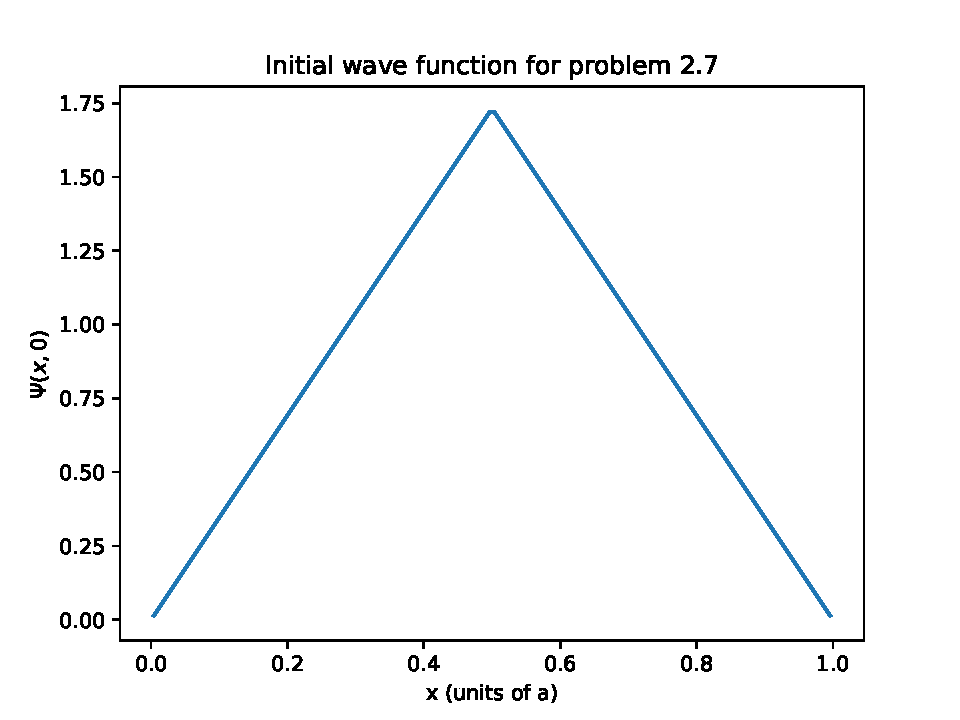
\includegraphics[width=0.7\textwidth]{./res/Prblm2.pdf}
    \caption{Sketch of the initial wave function Eq.~\eqref{eq:Prblm2WaveFunction}.}
    \label{fig:Prblm2WaveFunction}
\end{figure}



\item The full solution is given by:

\begin{equation*}
    \Psi(x,t) = \sum_n c_n \psi_n(x),
\end{equation*}

but to find the $c_n$'s, we know by the completeness of the stationary states that we can also express the initial wavefunction as a linear combination of the stationary states:

\begin{equation*}
    \Psi(x,0) = \sum_n c_n \psi_n(x),
\end{equation*}

where these $c_n$'s would be different, of course, and the stationary states are given by

\begin{equation*}
    \psi_n = \sqrt{\frac{2}{a}}\sin\left( \frac{n\pi x}{a} \right).
\end{equation*}

We can then invoke tactics from Fourier analysis to find the coefficients:

\begin{equation*}
    c_n = \int \psi_n \Psi(x,0) \;\ddx = \sqrt{\frac{12}{a^3}}\sqrt{\frac{2}{a}} \left[ \int_0^{a/2} x\sin\left( \frac{n\pi x}{a} \right)\;\ddx + \int_{a/2}^a (a-x)\sin\left( \frac{n\pi x}{a} \right)\;\ddx \right].
\end{equation*}

Looking at the first integral:

\begin{align*}
    \int_0^{a/2} x\sin\left( \frac{n\pi x}{a} \right)\;\ddx &= \left[ -\frac{ax}{n\pi}\cos\left( \frac{n\pi x}{a} \right)_0^{a/2} \right] + \frac{a}{n\pi}\int_0^{a/2} \cos\left( \frac{n\pi x}{a} \right)\;\ddx, \\
    &= -\frac{a^2}{2n\pi}\cos\left( \frac{n\pi}{2} \right) + \frac{a^2}{n^2\pi^2}\left[ \sin\left( \frac{n\pi x}{a} \right) \right]_0^{a/2}, \\
    &= -\frac{a^2}{2n\pi}\cos\left( \frac{n\pi}{2} \right) + \frac{a^2}{n^2\pi^2}\sin\left( \frac{n\pi}{2} \right).
\end{align*}

Now for the second integral:

\begin{equation*}
    \int_{a/2}^a (a-x)\sin\left( \frac{n\pi x}{a} \right)\;\ddx = a\int_{a/2}^a \sin\left( \frac{n\pi x}{a} \right)\;\ddx - \int_{a/2}^a x\sin\left( \frac{n\pi x}{a} \right)\;\ddx.
\end{equation*}

We can use the results of the previous integral for the second integral here:

\begin{align*}
    &= -\frac{a^2}{n\pi}\left[ \cos\left( \frac{n\pi x}{a} \right) \right]_{a/2}^a - \left\{ \left[ -\frac{ax}{n\pi}\cos\left( \frac{n\pi x}{a} \right) \right]_{a/2}^a + \frac{a^2}{n^2\pi^2}\left[ \sin\left( \frac{n\pi x}{a} \right) \right]_{a/2}^a \right\}, \\
    &= -\frac{a^2}{n\pi} \left[ \cos(n\pi) - \cos\left( \frac{n\pi}{2} \right) \right] - \left\{ -\frac{a^2}{n\pi}\cos(n\pi) + \frac{a^2}{2n\pi}\cos\left( \frac{n\pi}{2} \right) + \frac{a^2}{n^2\pi^2}\left[ \sin(n\pi) - \sin\left( \frac{n\pi}{2} \right) \right] \right\}, \\
    &= -\frac{a^2}{n\pi}\cos\left( \frac{n\pi}{2} \right) + \frac{a^2}{n\pi}\cos\left( \frac{n\pi}{2} \right) + \frac{a^2}{n\pi}\cos(n\pi) - \frac{a^2}{2n\pi}\cos\left( \frac{n\pi}{2} \right) + \frac{a^2}{n^2\pi^2}\sin\left( \frac{n\pi}{2} \right), \\
    &= \frac{a^2}{2n\pi}\cos\left( \frac{n\pi}{2} \right) + \frac{a^2}{n^2\pi^2}\sin\left( \frac{n\pi}{2} \right).
\end{align*}

Adding this with the previous integral gets us:

\begin{equation*}
    -\frac{a^2}{2n\pi}\cos\left( \frac{n\pi}{2} \right) + \frac{a^2}{n^2\pi^2}\sin\left( \frac{n\pi}{2} \right) + \frac{a^2}{2n\pi}\cos\left( \frac{n\pi}{2} \right) + \frac{a^2}{n^2\pi^2}\sin\left( \frac{n\pi}{2} \right) = \frac{2a^2}{n^2\pi^2}\sin\left( \frac{n\pi}{2} \right).
\end{equation*}

So,

\begin{equation*}
    c_n = \sqrt{\frac{24}{a^4}} \cdot \frac{2a^2}{n^2\pi^2}\sin\left( \frac{n\pi}{2} \right) = \frac{4\sqrt{6}}{n^2\pi^2}(-1)^{(n+1)/2},
\end{equation*}

where this is only valid for odd $n$. Therefore,

\begin{equation*}
    \boxed{\Psi(x,t) = \frac{4\sqrt{6}}{\pi^2}\sqrt{\frac{2}{a}} \sum_{n=1,3,5,\ldots} \frac{(-1)^{(n+1)/2}}{n^2} \sin\left( \frac{n\pi x}{a} \right) e^{-i(n^2\pi^2\hbar/2ma^2)t}.}
\end{equation*}



\item We know that such a probability is equal to $\abs{c_n}^2$, so:

\begin{equation*}
    P(E = E_1) = \left( \frac{4\sqrt{6}}{\pi^2} \right)^2 \approx \boxed{0.9855.}
\end{equation*}




\item The expectation value of the energy is:

\begin{equation}
    \Braket{H} = \sum_n \abs{c_n}^2 E_n = \left( \frac{4\sqrt{6}}{n^2\pi^2} \right)^2 \frac{n^2\pi^2\hbar^2}{2ma^2} = \frac{48\hbar^2}{m\pi^2a^2} \sum_{n=1,3,5,\ldots} \frac{1}{n^2}.
\end{equation}

I looked up the series, it turns out is is equal to $\pi^2/8$, so:

\begin{equation*}
    \boxed{\Braket{H} = \frac{6\hbar^2}{ma^2}.}
\end{equation*}




\end{parts}